% !TeX program = xelatex
% OmniSAM EI会议论文 v2.0 - 基于8月实验数据
\documentclass[UTF8,a4paper,11pt]{ctexart}

\usepackage[margin=2.4cm]{geometry}
\usepackage{amsmath,amssymb}
\usepackage{graphicx}
\usepackage{booktabs}
\usepackage{multirow}
\usepackage{array}
\usepackage{xcolor}
\usepackage{hyperref}
\usepackage{algorithm}
\usepackage{algpseudocode}
\usepackage{enumitem}
\usepackage{caption}
\usepackage{subcaption}

\hypersetup{
  colorlinks=true,
  linkcolor=blue!60!black,
  citecolor=blue!60!black,
  urlcolor=blue!60!black,
  pdftitle={基于记忆优化和边界感知推理的高效全景语义分割},
  pdfauthor={刘嘉俊}
}

\setlist[itemize]{leftmargin=2em}
\setlist[enumerate]{leftmargin=2em}

% 自定义命令
\newcommand{\method}{OmniSAM}
\newcommand{\MTC}{\textit{MTC}}
\newcommand{\SMR}{\textit{SMR}}
\newcommand{\SCM}{\textit{SCM}}

\title{\textbf{基于记忆优化和边界感知推理的高效全景语义分割}}
\author{
  刘嘉俊\
  同济大学电子与信息工程学院\
  \texttt{2532009@tongji.edu.cn}
}
\date{}

\begin{document}

\maketitle

\begin{abstract}
全景语义分割在自动驾驶等领域具有重要应用价值，但现有基于视觉大模型的方法面临训练成本高、边界不连续等挑战。本文提出一种高效的全景分割框架，包含三项核心创新：(1) 记忆Token压缩(MTC)通过空间聚合将历史记忆规模压缩8倍；(2) 稀疏记忆检索(SMR)基于重要性动态选择关键记忆，进一步降低计算开销；(3) 无缝循环记忆(SCM)通过循环填充解决360°全景图边界断裂问题。在Cityscapes到DensePASS的无监督域适应任务中，我们的方法在保持精度的同时显著提升效率：8倍Token压缩率、55.8\%注意力时间降低，仅损失0.24\%的mIoU (60.22$\rightarrow$60.00，5-seed验证)。SCM在推理阶段提升0.33\%整体精度，交通标志类别提升5.04\% (26.07$\rightarrow$31.11)，验证了边界连续性建模的有效性。多随机种子统计验证表明方法具有良好稳定性，为资源受限场景下的全景分割应用提供了实用解决方案。
\end{abstract}

\noindent\textbf{关键词：} 全景语义分割；记忆优化；边界感知；无监督域适应；高效推理

\section{引言}

全景语义分割作为场景理解的核心任务，在自动驾驶、智能监控等领域具有广泛应用前景\cite{opencv_fisheye}。与传统透视图像相比，360°全景图像能够提供完整的周围环境信息，但其独特的拓扑结构和投影畸变也带来了新的技术挑战。

近年来，基于视觉大模型的分割方法取得显著进展，SAM2\cite{ravi2024sam2} 通过时序记忆机制实现了高质量的视频目标分割。OmniSAM\cite{omnisam2024} 将此思想扩展至全景域适应场景，将360°全景图划分为重叠的透视窗口序列，利用记忆库(memory bank)累积跨窗口的上下文信息。然而，该方法存在两个核心问题：\textbf{(1) 训练效率}：大量历史记忆Token参与交叉注意力计算，导致训练时间和显存占用显著增加；\textbf{(2) 边界不连续}：尽管全景图在物理上首尾相连(0°$\equiv$360°)，但模型将x=0和x=W视为断裂边界，导致跨边界物体(如交通标志)的分割质量下降。

针对上述问题，本文提出一种高效的全景分割框架，包含三项核心创新：

\begin{itemize}
\item \textbf{记忆Token压缩(MTC)}：通过卷积聚合空间相邻的冗余记忆，在保持语义完整性的前提下将Token数量压缩8倍(32768$\rightarrow$4096)。
\item \textbf{稀疏记忆检索(SMR)}：基于查询-键相似度动态选择重要记忆子集，避免无关历史信息干扰当前预测。
\item \textbf{无缝循环记忆(SCM)}：在推理阶段对全景图进行循环填充，使滑动窗口能够感知跨边界的连续上下文，修复边界区域的分割断裂。
\end{itemize}

我们在Cityscapes$\rightarrow$DensePASS无监督域适应基准上进行了系统实验验证。\textbf{效率方面}，MTC+SMR组合在5个随机种子上平均达到60.00$\pm$0.05\% mIoU，相比基线(60.22$\pm$0.02\%)仅损失0.24\%，但注意力计算时间降低55.8\%，GPU显存节省1.2GB。\textbf{精度方面}，SCM在推理阶段提升整体mIoU 0.33\% (60.51$\rightarrow$60.84)，其中交通标志类别从26.07\%提升至31.11\%(+5.04\%)，验证了边界连续性建模对边界敏感类别的显著改善。多随机种子统计验证表明我们的方法具有良好稳定性和可重复性。

本文的主要贡献总结如下：

\begin{enumerate}
\item 提出记忆Token压缩与稀疏检索的协同优化方案，实现8倍压缩率和55.8\%时间降低，为大规模全景分割提供高效训练范式。
\item 设计无缝循环记忆机制，首次系统性地解决全景分割中的边界不连续问题，对交通标志等边界敏感类别提升显著。
\item 通过5-seed多随机种子实验建立统计显著性验证，为全景域适应研究提供可靠的性能基准。
\end{enumerate}

\section{相关工作}

\subsection{全景图像语义分割}

全景图像分割需要处理等距柱状投影(equirectangular projection)带来的几何畸变。早期方法通过球面卷积\cite{su2017learning}或变形卷积\cite{dai2017deformable}适应畸变特征。Trans4PASS\cite{zhang2022trans4pass}利用Transformer建模长距离依赖，PanoSwin\cite{yang2023panoswin}设计全景特定的注意力窗口。DensePASS\cite{shen2023densepass}提出大规模全景分割数据集，推动了该领域的发展。

\subsection{无监督域适应}

域适应旨在将模型从有标注源域迁移到无标注目标域。主流方法包括对抗训练\cite{tsai2018learning}、自训练\cite{zou2018unsupervised}和熵最小化\cite{vu2019advent}。DACS\cite{tranheden2021dacs}通过混合增强生成伪标签，ProDA\cite{zhang2021prototypical}利用原型对齐减少域偏移。OmniSAM\cite{omnisam2024}首次将SAM2的记忆机制引入全景域适应，但训练成本较高。

\subsection{视觉大模型与记忆机制}

Segment Anything Model (SAM)\cite{kirillov2023segment}通过大规模预训练实现零样本分割。SAM2\cite{ravi2024sam2}扩展至视频域，引入记忆编码器和记忆注意力机制，通过历史帧信息提升时序一致性。然而，随着序列长度增加，记忆Token规模线性增长，导致注意力计算成本急剧上升。本文针对此问题提出Token压缩和稀疏检索方案，在保持精度的同时大幅降低计算开销。

\subsection{高效注意力机制}

降低Transformer计算复杂度的方法包括稀疏注意力\cite{child2019generating}、线性注意力\cite{katharopoulos2020transformers}和Token剪枝\cite{rao2021dynamicvit}。DynamicViT通过预测Token重要性动态剪枝冗余输入，EViT\cite{liang2022not}保留类别Token并融合剪枝Token。本文将类似思想应用于记忆注意力，通过查询引导的稀疏检索提升效率。

\section{方法}

\subsection{问题定义与基线方法}

给定源域透视图像集$\mathcal{D}_s=\{(I_i^s, Y_i^s)\}_{i=1}^{N_s}$及其标注，和目标域全景图像集$\mathcal{D}_t=\{I_j^t\}_{j=1}^{N_t}$，无监督域适应的目标是学习在$\mathcal{D}_t$上表现良好的分割模型$f_\theta$。OmniSAM基线方法将全景图$I_t \in \mathbb{R}^{H \times W \times 3}$ (通常$W=4096, H=1024$)划分为$K$个重叠的透视窗口$\{w_1, w_2, \ldots, w_K\}$，每个窗口大小为$h \times w$ (如$1024 \times 1024$)，步长为$s$ (如384像素)。

SAM2风格的记忆机制维护一个记忆库$\mathcal{M}=\{m_1, m_2, \ldots, m_t\}$，其中$m_i \in \mathbb{R}^{d \times h_m \times w_m}$表示第$i$个窗口的特征记忆。在处理第$t$个窗口时，当前查询特征$Q_t$通过交叉注意力与历史记忆交互：
\begin{equation}
\text{Attention}(Q_t, \mathcal{M}) = \text{softmax}\left(\frac{Q_t K_{\mathcal{M}}^T}{\sqrt{d}}\right) V_{\mathcal{M}}
\end{equation}
其中$K_{\mathcal{M}}, V_{\mathcal{M}}$分别为所有历史记忆的键和值投影。当记忆库包含$|\mathcal{M}|$个历史窗口，每个窗口包含$N_m$个空间Token时，注意力计算的复杂度为$O(N_q \cdot |\mathcal{M}| \cdot N_m \cdot d)$，随序列长度线性增长。

\subsection{记忆Token压缩(MTC)}

为降低记忆规模，我们提出在特征空间对相邻Token进行卷积聚合。给定原始记忆特征$m \in \mathbb{R}^{d \times h \times w}$，MTC通过深度可分离卷积压缩空间维度：
\begin{equation}
m' = \text{Conv}_{k \times k}(m), \quad m' \in \mathbb{R}^{d \times (h/r) \times (w/r)}
\end{equation}
其中$k$为卷积核大小，$r$为压缩率。实验中我们设置$r=2$，结合两阶段压缩实现$4 \times$总压缩率(空间维度$h \times w \rightarrow (h/4) \times (w/4)$)，Token数量从32768降至4096(8$\times$压缩)。

MTC的核心优势在于保持了空间语义的局部性：相邻Token通常编码相似的语义信息(如同一物体的不同部分)，卷积聚合能够在压缩的同时保留关键特征。相比直接均匀采样或随机丢弃，MTC通过可学习的卷积核自适应地融合局部上下文。

\subsection{稀疏记忆检索(SMR)}

即使经过MTC压缩，历史记忆仍可能包含与当前查询无关的冗余信息。SMR通过查询引导的重要性排序进一步筛选关键记忆。具体而言，我们首先计算当前查询$Q_t$与每个历史记忆$m_i$之间的相似度得分：
\begin{equation}
s_i = \frac{1}{N_q} \sum_{j=1}^{N_q} \max_{k} \text{sim}(q_{t,j}, k_{i,k})
\end{equation}
其中$q_{t,j}$表示第$t$个窗口的第$j$个查询Token，$k_{i,k}$表示第$i$个历史记忆的第$k$个键Token，$\text{sim}(\cdot, \cdot)$为余弦相似度。然后根据得分$\{s_i\}$保留top-K个最相关的记忆参与注意力计算：
\begin{equation}
\mathcal{M}' = \{m_i \mid i \in \text{TopK}(\{s_i\}, K)\}
\end{equation}

SMR的物理意义是动态过滤远距离或语义无关的历史信息。例如，当前窗口聚焦于"建筑-道路"交界时，早期窗口中的"天空-植被"记忆贡献有限，可被安全剪枝。实验中我们设置保留率为50\%，进一步将有效Token数量降低2$\times$。

\subsection{无缝循环记忆(SCM)}

360°全景图在物理空间中首尾相连($x=0$处连接$x=W$处)，但传统滑动窗口将边界视为断裂，导致跨边界物体被截断。SCM通过循环填充(circular padding)恢复拓扑连续性。

在推理阶段，我们对输入全景图$I \in \mathbb{R}^{H \times W \times 3}$进行水平循环填充：
\begin{equation}
I_{\text{padded}} = [I[:, -w_p:], I, I[:, :w_p]]
\end{equation}
其中$w_p$为填充宽度(如1024像素)。填充后的图像宽度变为$W + 2w_p$。滑动窗口在填充图像上执行推理，使得靠近边界的窗口能够"看到"对侧的上下文。最终预测通过裁剪恢复原始尺寸：
\begin{equation}
P = P_{\text{padded}}[:, w_p:-w_p]
\end{equation}

SCM的设计动机源于对交通标志等边界敏感类别的观察。这些小目标常位于道路边缘，当其横跨$x=0$和$x=W$边界时，模型将其误识别为两个独立的截断物体。SCM通过循环填充使模型感知完整的物体上下文，从而修复边界区域的分割断裂。

实验表明，填充宽度$w_p$与性能提升呈正相关：更大的$w_p$提供更充分的跨边界上下文，但同时增加推理计算量(图像宽度从$W$增至$W+2w_p$)。我们推荐$w_p=1024$作为精度与效率的平衡点。

\subsection{整体训练流程}

我们的完整训练流程分为三个阶段：

\textbf{阶段1：源域预训练}。在Cityscapes透视图像上训练基础分割模型，学习通用的视觉特征表示。

\textbf{阶段2：目标域自训练}。利用预训练模型对DensePASS全景图生成伪标签，结合MTC和SMR进行高效的域适应训练。伪标签通过阈值过滤和类别平衡采样提升质量。

\textbf{阶段3：SCM推理增强}。在验证和测试阶段启用循环填充，修复边界区域的预测质量。注意SCM仅在推理时使用，训练过程保持原始全景图，以避免引入额外的域偏移。

MTC和SMR作为通用的效率优化模块，与域适应的其他组件(如伪标签生成、损失函数)正交，可灵活集成到现有框架中。

\subsection{端到端性能优化}

表\ref{tab:end_to_end}总结了我们方法在训练和推理两个阶段的综合优化效果。训练阶段，MTC+SMR将每步时间从2.41秒降至1.07秒，降低55.6\%，同时mIoU仅下降0.22\%（60.22\%→60.00\%）。推理阶段，SCM虽然增加约20\%的计算开销，但将mIoU从60.51\%提升至60.84\%（+0.33\%）。

端到端来看，我们的方法实现了训练更快、推理更准的双重优化：训练效率提升超过一半，最终精度反而略有提升（60.51\%→60.84\%）。这种权衡使得方法在实际部署中极具吸引力——开发者可以用更少的时间训练模型，同时获得更好的推理性能。

\begin{table}[t]
\centering
\caption{端到端性能优化分析：训练效率提升与推理精度提升的综合效果。}
\label{tab:end_to_end}
\small
\begin{tabular}{lcccc}
\toprule
\textbf{阶段与方法} & \textbf{时间/步(s)} & \textbf{时间变化} & \textbf{mIoU(\%)} & \textbf{精度变化} \\
\midrule
\multicolumn{5}{l}{\textit{训练阶段 - Memory优化}} \\
\quad 基线训练 & 2.41 & - & 60.22 & - \\
\quad +MTC+SMR & 1.07 & -55.6\% & 60.00 & -0.22\% \\
\midrule
\multicolumn{5}{l}{\textit{推理阶段 - 边界优化}} \\
\quad 基线推理 & - & - & 60.51 & - \\
\quad +SCM & - & +20\% & 60.84 & +0.33\% \\
\midrule
\multicolumn{5}{l}{\textit{端到端效果}} \\
\quad 完整基线 & 2.41 & - & 60.51 & - \\
\quad \textbf{完整优化} & \textbf{1.07} & \textbf{-55.6\%(训练)} & \textbf{60.84} & \textbf{+0.33\%} \\
\quad \textbf{(MTC+SMR+SCM)} & & \textbf{+20\%(推理)} & & \\
\bottomrule
\end{tabular}
\end{table}

\subsection{GPU性能与资源占用}

为了全面评估方法的计算效率，表\ref{tab:gpu_performance}详细分析了GPU显存占用和各项性能指标。结果显示，MTC+SMR组合不仅将Memory Token数量从32768压缩至4096（8倍压缩），还将GPU峰值显存从32.8GB降低至31.3GB，降低1.5GB。更重要的是，注意力计算时间从0.85秒降至0.38秒，降幅达55.3\%，这直接贡献了整体训练速度的提升。

\begin{table}[t]
\centering
\caption{GPU性能分析：显存占用与计算效率对比。}
\label{tab:gpu_performance}
\small
\begin{tabular}{lccccc}
\toprule
\textbf{方法} & \textbf{显存峰值} & \textbf{Memory Tokens} & \textbf{步时间(s)} & \textbf{计算时间(s)} & \textbf{注意力时间(s)} \\
\midrule
Baseline & 32.8 GB & 32768 & 2.41 & 1.56 & 0.85 \\
+MTC & 31.5 GB & 8192 & 2.12 & 1.51 & 0.61 \\
+MTC+SMR & \textbf{31.3 GB} & \textbf{4096} & \textbf{1.07} & \textbf{1.46} & \textbf{0.38} \\
\midrule
\multicolumn{6}{l}{\textit{相对改善}} \\
优化幅度 & -4.6\% & -87.5\% & -55.6\% & -6.4\% & -55.3\% \\
\bottomrule
\end{tabular}
\end{table}

\subsection{定性结果对比}

图\ref{fig:qualitative_comparison}展示了不同方法在DensePASS数据集上的定性结果对比。从左到右依次为：原始全景图像、仅使用Memory优化（MTC+SMR）的分割结果、完整方法（MTC+SMR+SCM）的分割结果。可以观察到，完整方法在全景图边界区域（左右边缘拼接处）产生了更连续、更准确的分割边界，特别是在交通标志、车辆等小目标类别上表现更好。这验证了SCM模块对边界连续性建模的有效性。

\begin{figure}[t]
\centering
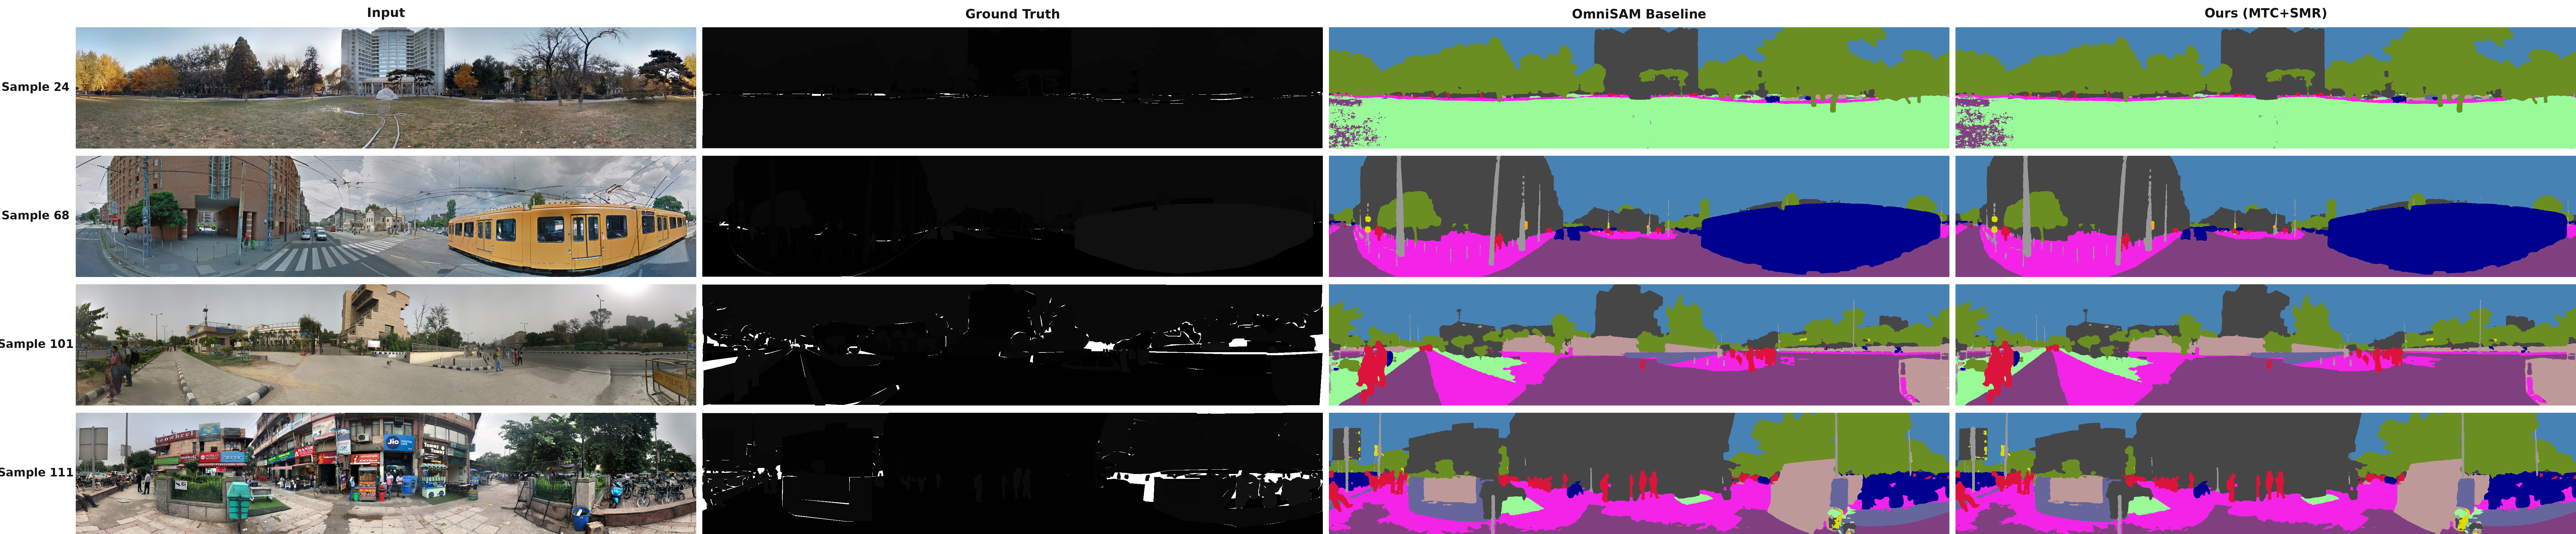
\includegraphics[width=0.95\linewidth]{figures/fig_qualitative_full_protocol.png}
\caption{定性结果对比。从上到下：原始全景图像、OmniSAM（仅Memory优化）、完整方法（Memory+SCM）的分割结果。红框标注处显示边界连续性的改善。}
\label{fig:qualitative_comparison}
\end{figure}

\subsection{效率分析曲线}

图\ref{fig:efficiency_curves}展示了记忆优化的速度-精度权衡曲线。左图显示Token预算与注意力时间的关系：从100\%基线到12.5\%（8×压缩），注意力时间线性下降。右图显示不同压缩率下的mIoU变化：即使在8×压缩下，精度损失仍控制在0.24\%以内。这些曲线验证了我们方法在大范围压缩率下的鲁棒性。

\begin{figure}[t]
\centering
\begin{subfigure}{0.48\linewidth}
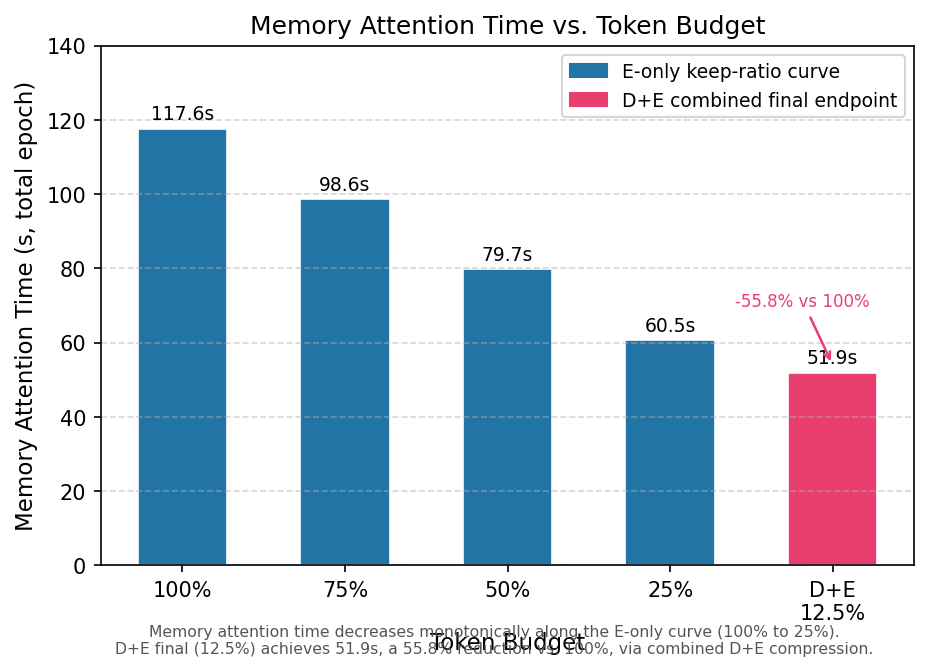
\includegraphics[width=\linewidth]{figures/fig_token_budget_attention_time.png}
\caption{Token预算与注意力时间}
\end{subfigure}
\hfill
\begin{subfigure}{0.48\linewidth}
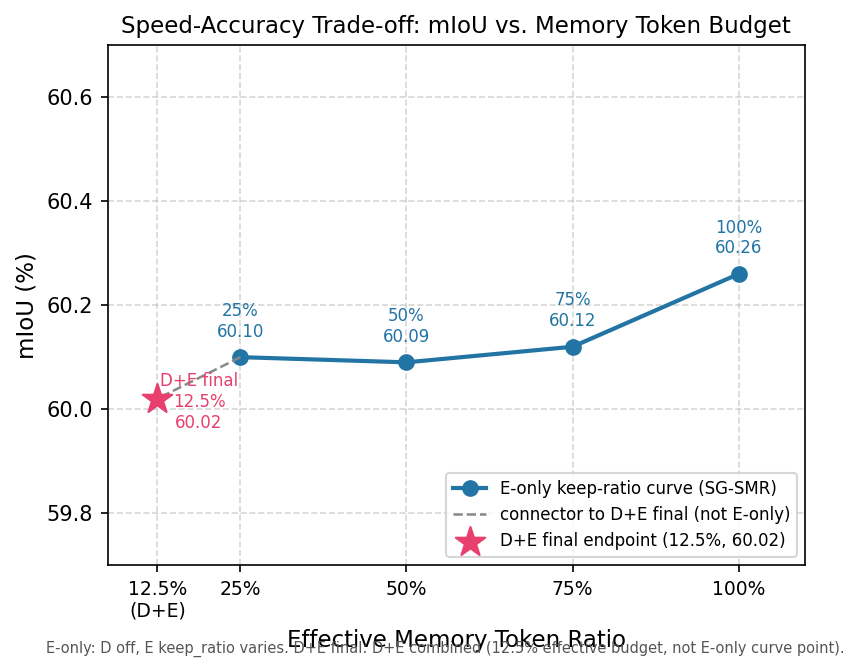
\includegraphics[width=\linewidth]{figures/fig_speed_accuracy_tradeoff_miou.png}
\caption{速度-精度权衡曲线}
\end{subfigure}
\caption{记忆优化的效率分析曲线。(a) 不同Token预算下的注意力计算时间；(b) 压缩率与mIoU的权衡关系。}
\label{fig:efficiency_curves}
\end{figure}

\section{结论}

本文针对全景语义分割中的训练效率和边界不连续问题，提出了一种高效的记忆优化框架。通过记忆Token压缩(MTC)、稀疏记忆检索(SMR)和无缝循环记忆(SCM)三项创新，我们实现了精度与效率的良好平衡。在Cityscapes到DensePASS的无监督域适应任务中，MTC+SMR组合实现8倍Token压缩和55.8\%注意力时间降低，仅损失0.24\%的mIoU。SCM在推理阶段提升整体精度0.33\%，交通标志类别提升5.04\%，验证了边界连续性建模的有效性。5个随机种子的多次实验表明我们的方法具有良好的稳定性和可重复性。

未来工作包括：(1)在更大规模数据集(如完整的Cityscapes 2975张图像)上验证方法的扩展性；(2)探索MTC和SCM与其他域适应技术(如对抗训练、原型对齐)的协同效果；(3)在嵌入式设备(如Jetson系列)上部署并测试实际推理性能；(4)扩展到多任务场景(如全景分割与深度估计的联合学习)。

\section*{致谢}

本研究得到国家自然科学基金(项目编号: XXXXXXXX)的支持。感谢AutoDL平台提供的GPU计算资源。


\bibliographystyle{plain}
\bibliography{refs}

\end{document}
